\chapter{Continuity Equation}
\label{ch:continuity}

\section{Learning objectives}
At the end of this chapter, a student should be able to 
\begin{enumerate}
\item apply continuity equation to determine unknown components of a velocity field
\item plot stream function as contours to visualize flow field in a 2D domain
\end{enumerate}

% learning objective
\begin {lo3} [Fluid Flow]
Derive continuity equation
\end {lo3}

\section{Concept map}
\index{Concept map, material derivative}

\begin{figure}[h]
\begin{center}
\framebox{
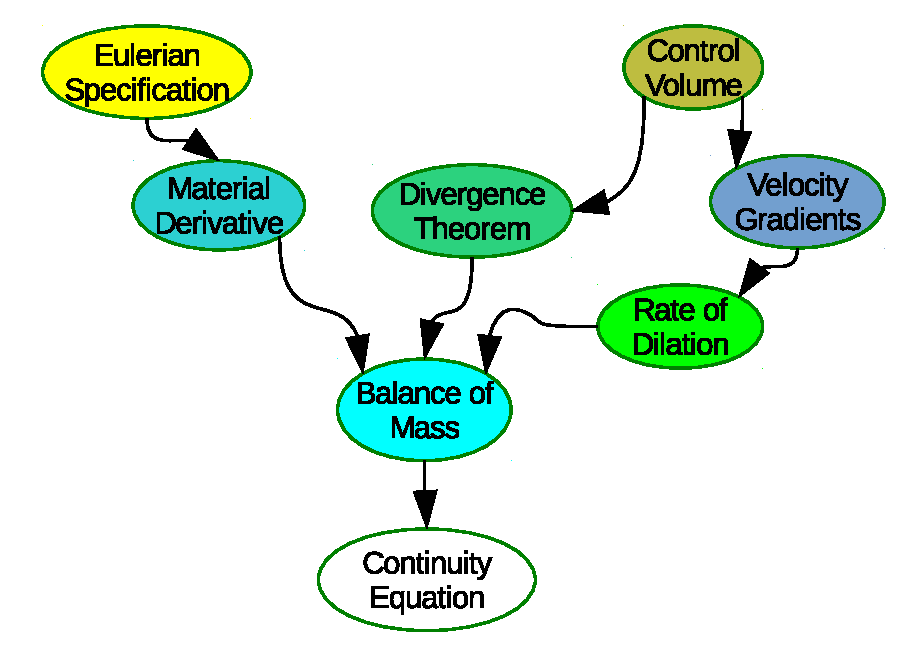
\includegraphics[scale=0.8]{images/c07-MaterialDerivativeFlowChart.eps}
 }
\end{center}
\caption{Concept map to arrive at continuity equation}
\label{ContinuityEquationConceptMap}
\end{figure}

A concept map that exposes the connections between different concepts behind continuity equation is given in the figure~\ref{ContinuityEquationConceptMap}.

% -----------------------------------------------------------------------

\section{Type of specifications}

\begin{figure}[h]
\begin{center}
\framebox{
\includegraphics[scale=0.8]{images/c07-eulerlagrange.eps}
 }
\end{center}
\caption{An image generated by chatgpt to show Euler as traffic police and Lagrange as a driver. Helps connect the specifications to the respective perspectives}
\label{eulerlagrange}
\end{figure}


Figure~\ref{VolumeElementMotion} illustrates a control volume being advected in a fluid. Consider a parameter that can be specified at the center of this control volume. Time derivative of such a parameter could be described either in a coordinate system fixed to the center of the control volume itself or in an external coordinate system of the observer.

\begin{figure}[h]
\begin{center}
\framebox{
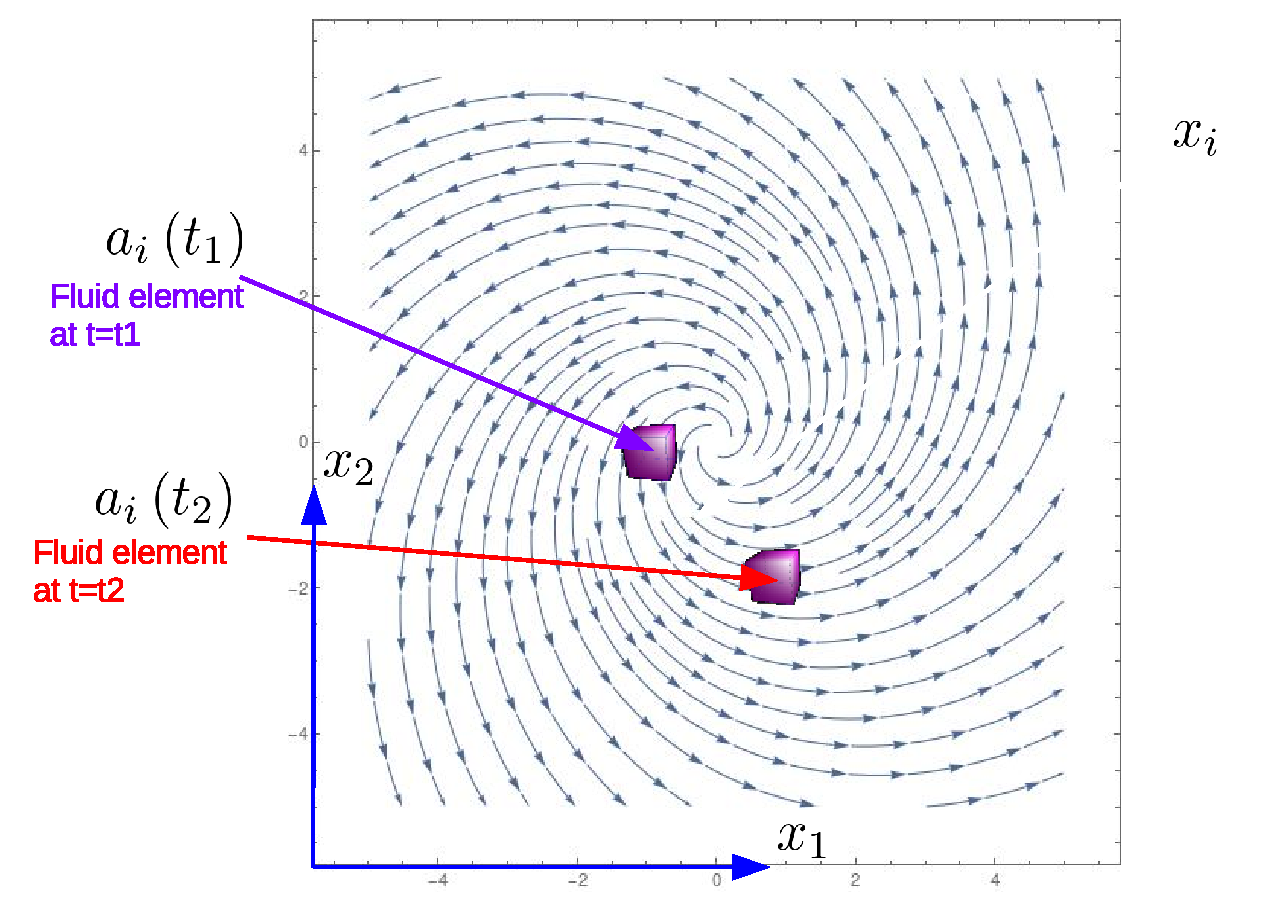
\includegraphics[scale=0.5]{images/c07-VolumeElementMotion.eps}
 }
\end{center}
\caption{Motion of a volume element in a fluid}
\label{VolumeElementMotion}
\end{figure}


% -----------------------------------------------------------------------


{\bf Lagrangian}:
Velocities are specified at the centre of mass ($a_i$) and time ($t$).

{\bf Eulerian}:
Velocities are specified in terms of position ($x_i$) and time ($t$).

\begin{itemize}
\item Eulerian specification gives spatial gradients of velocities directly.
\item Lagrangian specification helps trace the path of an element directly.
\end{itemize}


% -----------------------------------------------------------------------

\section{Time derivative}

\index{Eulerian specification}
Consider a flow field and trace a particle that moves with the flow. The flow field can be specified in two ways. In the {\bf Eulerian} type of specification, the velocities are specified in terms of position ($x_i$) and time ($t$). It gives the spacial distribution of velocity $u_i(x_i,t)$ similar to density, temperature and pressure at any given instant. 

\index{Lagrangian specification}
In {\bf Lagrangian} type of specification, the dynamical history of a specific piece of material (fluid element) is given. The flow field of the element is given in terms of the position (of the center of mass) of the element and time as $v_i(a_i,t)$. 

Eulerian specification gives spacial gradients of velocities directly. Lagrangian specification helps trace the path of an element directly. Unless otherwise specified, one usually uses to the Eulerian frame of reference.

In the Lagrangian specification, since the velocity $v_i(a_i, t)$ is specified at the centre of gravity of the fluid element, acceleration of a fluid element is given by

\begin{equation}
\frac{dv_i}{dt} = \frac{\partial v_i}{\partial t} 
\end{equation} 

In the Eulerian specification, since the velocity ($u_i(x_i,t)$) is specified in terms of the absolute position where as the location of the fluid element changes as dictated by the flow  (see section \ref{variablechange}), acceleration of the fluid element is given as below:

\begin{equation}
\frac{du_i}{dt} = \frac{\partial u_i}{\partial t} + u_i \frac{\partial u_j}{\partial x_j} = \frac{\partial u_i}{\partial t} + u_j \nabla_j u_i 
\end{equation} 

or

\begin{equation}
\frac{d\vec{u}}{dt} = \frac{\partial \vec{u}}{\partial t} + (\vec{u} \cdot \vnabla) \vec{u} 
\end{equation} 

Proof of the same is given in section \ref{materialderivative}.

We now define the {\bf material derivative} which is a time derivative following the motion of the fluid as 

\begin{equation}
\boxed{\frac{D}{Dt} = \frac{\partial}{\partial t} + (\vec{u} \cdot \vnabla) }
\end{equation} 


{\bf Lagrangian}:
$$ {d \phi \over d t} = {\partial \phi \over \partial t} $$

{\bf Eulerian}:
$$ {d \phi \over d t} = {\partial \phi \over \partial t} +  {\partial \phi \over \partial x_1} {\partial x_1 \over \partial t} + {\partial \phi \over \partial x_2} {\partial x_2 \over \partial t} + {\partial \phi \over \partial x_3} {\partial x_3 \over \partial t} $$
$$ = {\partial \phi \over \partial t} +  {\partial \phi \over \partial x_1} u_1 + {\partial \phi \over \partial x_2} u_2 + {\partial \phi \over \partial x_3} u_3 $$
$$ = \left[ {\partial \over \partial t} +  u_1 {\partial \over \partial x_1} + u_2 {\partial \over \partial x_2} + u_3 {\partial \over \partial x_3} \right] \phi $$
$$ {d \phi \over d t} = \left[ {\partial \over \partial t} + \vec{u} \cdot \vec{\nabla} \right] \phi $$

% -----------------------------------------------------------------------

{\bf Acceleration}

{\bf Lagrangian}:
$$ {d \vec{V} \over d t} = {\partial \vec{V} \over \partial t} $$

{\bf Eulerian}:
$$ {d \vec{u} \over d t} = \left[ {\partial \over \partial t} + \vec{u} \cdot \vec{\nabla} \right] \vec{u} $$

% -----------------------------------------------------------------------


{\bf Material derivative}:

$$ {D \over D t} \equiv {\partial \over \partial t} + \vec{u} \cdot \vec{\nabla} \equiv {\partial \over \partial t} + u_j \nabla_j $$

% -----------------------------------------------------------------------

\section{Flux of mass}

{\bf Convention for flux}:

\begin{figure}[h]
\begin{center}
\framebox{
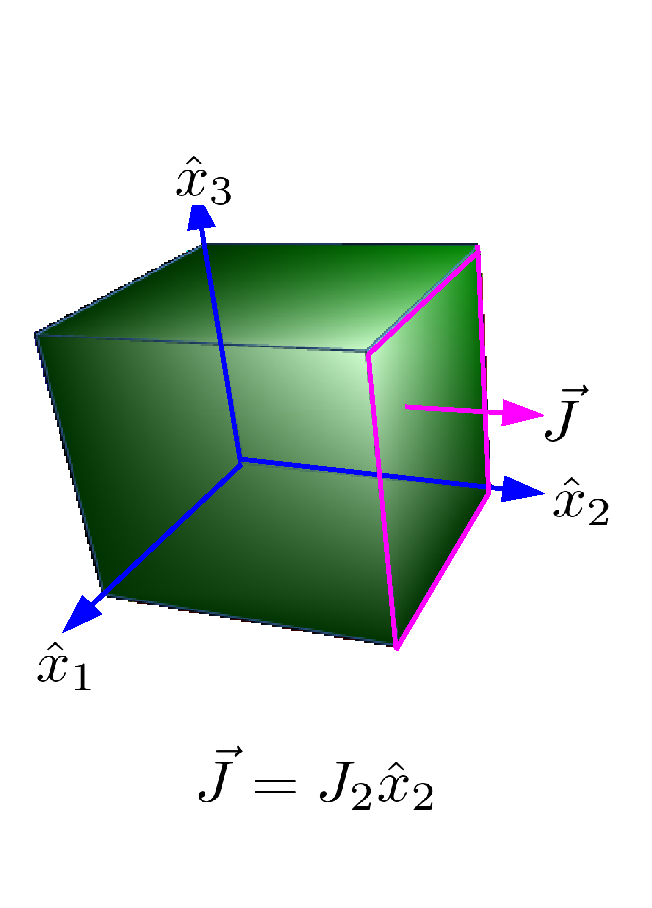
\includegraphics[scale=0.5]{images/c07-FluxConvention.eps}
 }
\end{center}
\caption{Convention for flux of material}
\label{FluxConvention}
\end{figure}


Area element has {\bf outward} normal.
$$ \vec{dS} = dA \, \hat{n} $$
$$ \vec{dS} = dx_1 \, dx_3 \, \hat{x}_2 $$
Mass flux:
$$ \vec{J} = \rho \vec{u} $$
$$ J_2 = \rho u_2 $$
Mass flow rate through the area element:
$$ \vec{J} \cdot \vec{dS} = \rho u_2 \, dx_1 \, dx_3 $$

% -----------------------------------------------------------------------

{\bf Divergence theorem}:

\begin{figure}[h]
\begin{center}
\framebox{
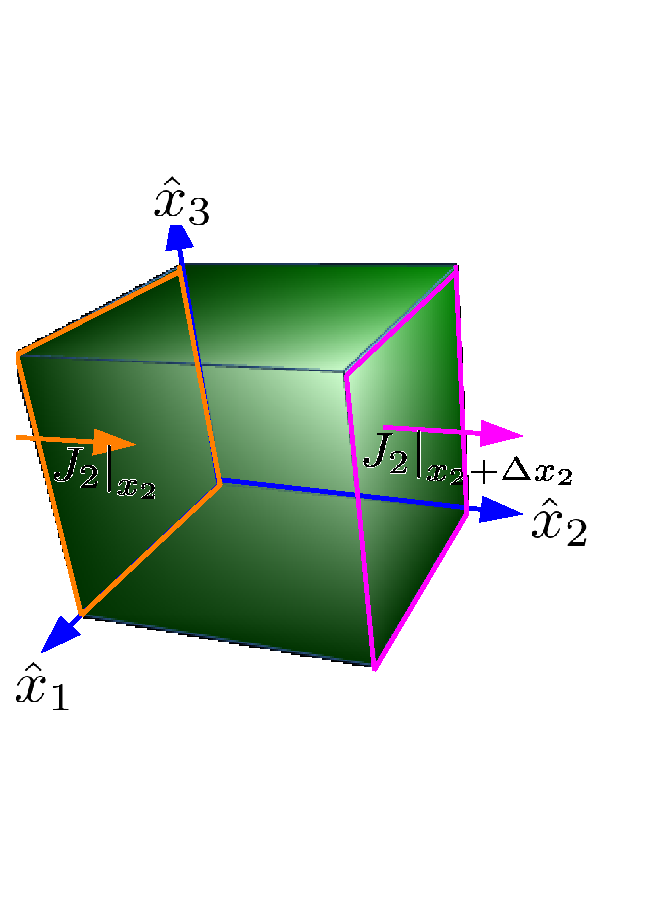
\includegraphics[scale=0.5]{images/c07-DivergenceTheorem.eps}
 }
\end{center}
\caption{Schematic for divergence theorem}
\label{DivergenceSchematic}
\end{figure}

Consider for 6 faces of the volume element:
$$ \sum{\vec{J} \cdot \vec{dS}} $$

Total outward mass flow:
$$ \left. J_2 \right|_{x_2+\Delta x_2} \Delta x_1 \Delta x_3 - \left. J_2 \right|_{x_2} \Delta x_1 \Delta x_3 $$
$$ + \left. J_3 \right|_{x_3+\Delta x_3} \Delta x_1 \Delta x_2 - \left. J_3 \right|_{x_3} \Delta x_1 \Delta x_2 $$
$$ + \left. J_1 \right|_{x_1+\Delta x_1} \Delta x_2 \Delta x_3 - \left. J_1 \right|_{x_1} \Delta x_2 \Delta x_3 $$
$$ = \left[ { \partial J_1 \over \partial x_1} + { \partial J_2 \over \partial x_2} + { \partial J_3 \over \partial x_3}  \right] \Delta x_1 \Delta x_2 \Delta x_3 $$
$$ \Delta V = \Delta x_1 \, \Delta x_2 \, \Delta x_3 $$


% -----------------------------------------------------------------------

{\bf Divergence theorem}:

$$ \sum{\vec{J} \cdot \vec{dS}} = \left[ \vec{\nabla} \cdot \vec{J} \right] \Delta V $$
$$ \int_{s}{\vec{J} \cdot \vec{dS}} = \int_{v}{\vec{\nabla} \cdot \vec{J} dV} $$ 
$$ \int_{s}{J_i \, n_i \, dS} = \int_{v}{ {\partial J_i \over \partial x_i} dV} $$ 

% -----------------------------------------------------------------------

\section{Mass balance}

{\bf Statement in words}:
Total influx of mass into a control volume equals increase in its mass.

As per our convention, $\vec{dS}$ is outward normal to the face of the control volume. So $\int_{s}{\vec{J} \cdot \vec{dS}}$ is total outflux.

Increase in mass of a control volume fixed in space is $\int_{v}{{\partial \rho \over \partial t} dV}$.

{\bf Statement for a CV }
$$\int_{v}{{\partial \rho \over \partial t} dV} = - \int_{s}{\vec{J} \cdot \vec{dS}}$$


% -----------------------------------------------------------------------

\section{Continuity equation}

Consider a control volume of surface area $S$ and volume $V$ though which a flow $\vec{u}$ is taking place. Conservation of mass requires that the increase in amount of fluid in the element is equal to the amount brought in by the fluid flow (in the absence of sources and sinks that are singular). By convention, the surface normal $\vec{n}$ points {\em outwards} and hence the conservation can be written as follows.

Mass balance over a control volume fixed in space:

\begin{equation}
	\int_{V}{\frac{\partial \rho}{\partial t} dV} = -\int_{S}{\vec{J} \cdot\vec{n}dS} = -\int_{S}{\left( \rho\vec{u} \right) \cdot\vec{n}dS}
\end{equation} 

$$ \int_{v}{{\partial \rho \over \partial t} dV} = - \int_{s}{\vec{J} \cdot \vec{dS}} = - \int_{v}{\vec{\nabla} \cdot \vec{J} dV} = - \int_{v}{\vec{\nabla} \cdot \left(\rho \vec{u} \right) dV} $$

Expanding the RHS,

$$ \int_{v}{{\partial \rho \over \partial t} dV} = - \rho \int_{v}{\vec{\nabla} \cdot \vec{u} dV} - \int_{v}{ \vec{u} \cdot \vec{\nabla} \rho dV} $$

$$ \int_{v}{\left[{\partial \rho \over \partial t} + \vec{u} \cdot \vec{\nabla} \rho\right] dV} = - \int_{v}{ \rho \vec{\nabla} \cdot \vec{u} dV} $$


Using the Gauss theorem\footnote{Actually Gauss-Ostrogradsky theorem} to convert the surface integral to volume integral,

\begin{equation}
\int_{V}{\frac{\partial \rho}{\partial t} dV} = -\int_{V}{\vnabla\cdot(\rho\vec{u})dV}
\end{equation} 

For this relation to be valid at {\em all} locations in the fluid,


\begin{equation}
\label{conteq1}
\boxed{\frac{\partial \rho}{\partial t} +  \vnabla\cdot(\rho\vec{u}) = 0}
\end{equation}


Use the identity in question~\ref{divsv} to expand the above equation as

\begin{equation}
\frac{\partial \rho}{\partial t} + (\vec{u}\cdot\vnabla)\rho + \rho\vnabla\cdot\vec{u}  = 0
\end{equation} 

Identifying the definition of material derivative $\frac{D}{Dt}$ and dividing by $\rho$,

\begin{equation}
\label{conteq2}
\boxed{\frac{1}{\rho}\frac{D \rho}{D t} + \vnabla\cdot\vec{u}  = \frac{1}{\rho}\frac{D \rho}{D t} + \Delta = 0}
\end{equation} 

\index{Rate of dilation}
\index{Compressibility}
\index{Rate of expansion}
$\vnabla\cdot\vec{u}$ is called as {\em rate of dilation} or rate of expansion or compressibility and is indicated by a symbol $\Delta$.

\begin{equation}
\label{rdiln}
\Delta = \vnabla\cdot\vec{u}  = \nabla_i u_i = u_{i,i}
\end{equation} 

Equations \ref{conteq1} and \ref{conteq2} are two alternate forms of the {\em continuity equation}.

\index{Incompressible fluid}
A fluid is called as {\em incompressible} if the density does not change due to changes in pressure (or) if the rate of change of density following the flow is zero. For {\em incompressible} fluids, the continuity equation reduces to:

\begin{equation}
\vnabla\cdot\vec{u}  = \Delta = 0
\end{equation} 

Sections \ref{variablechange} and \ref{materialderivative} state the same thing more rigorously.

% -----------------------------------------------------------------------

\section{Strain rate tensor}

The way velocity gradients would change the shape of a moving control volume in a fluid is illustrate in the following figures.

\begin{figure}[h]
\begin{center}
\framebox{
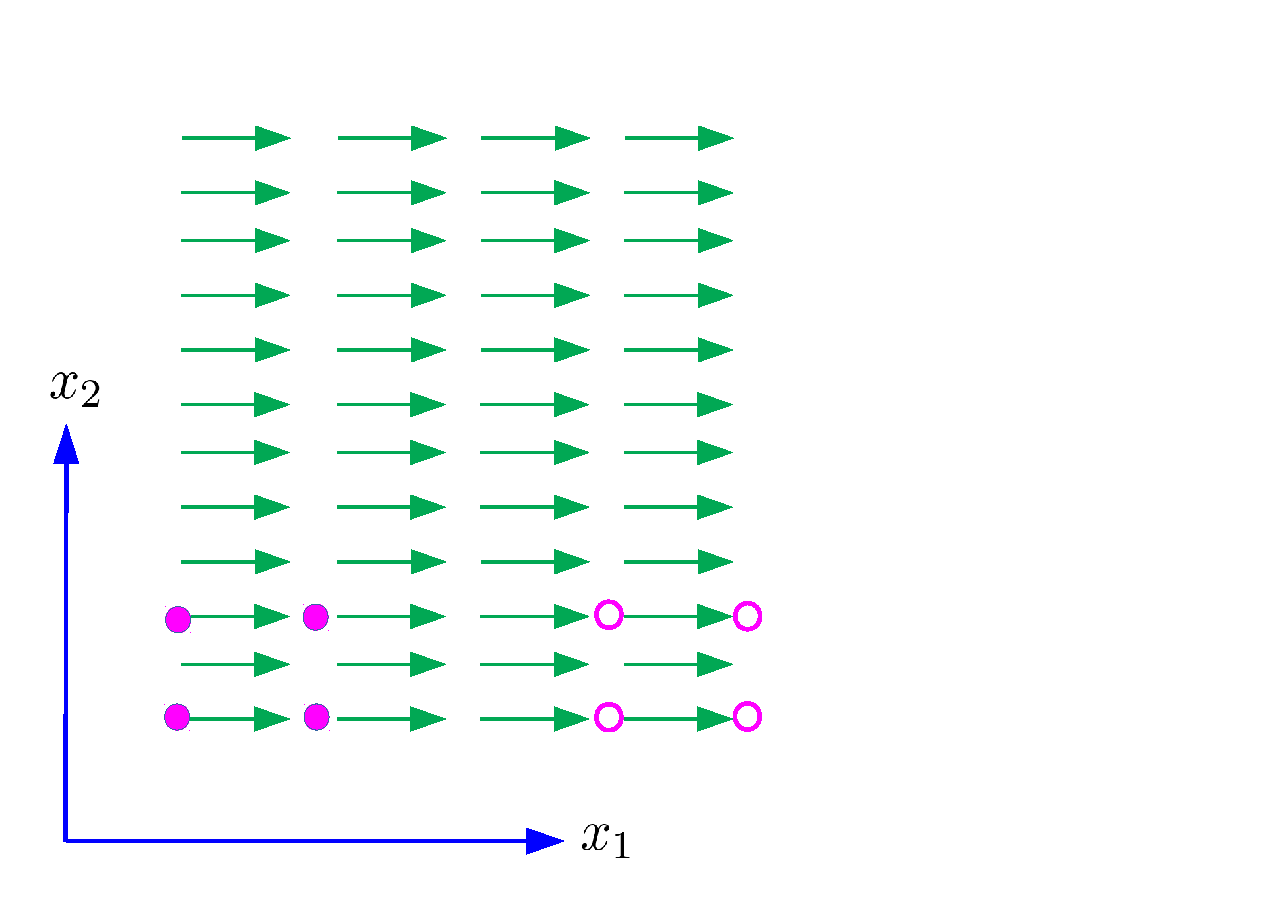
\includegraphics[scale=0.5]{images/c07-CVTranslate1.eps}
 }
\end{center}
\caption{Motion of a control volume due to unidirectional flow along $\hat{x}_1$}
\label{CVTranslation1}
\end{figure}


% -----------------------------------------------------------------------

\begin{figure}[h]
\begin{center}
\framebox{
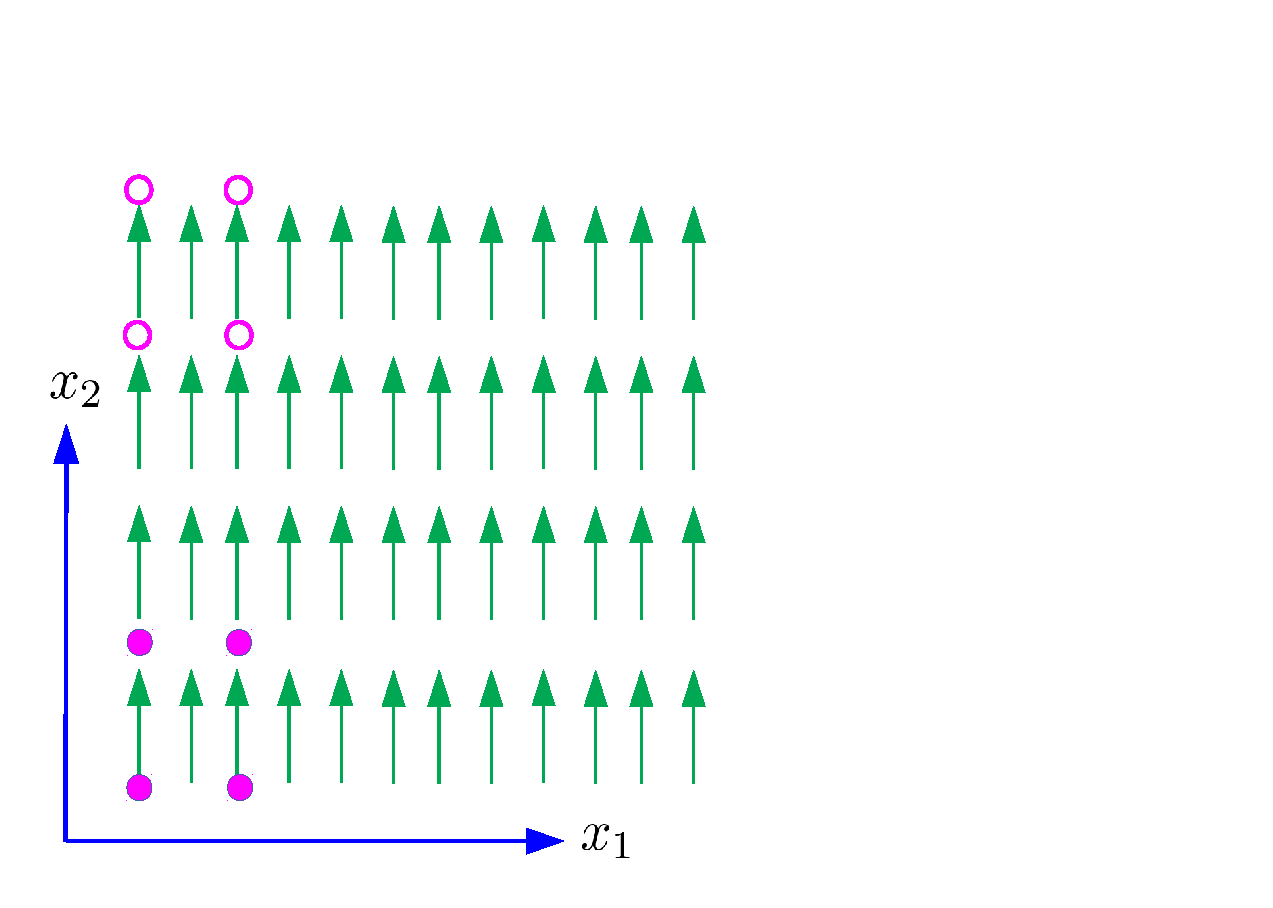
\includegraphics[scale=0.5]{images/c07-CVTranslate2.eps}
 }
\end{center}
\caption{Motion of a control volume due to unidirectional flow along $\hat{x}_2$}
\label{CVTranslation2}
\end{figure}


% -----------------------------------------------------------------------

\begin{figure}[h]
\begin{center}
\framebox{
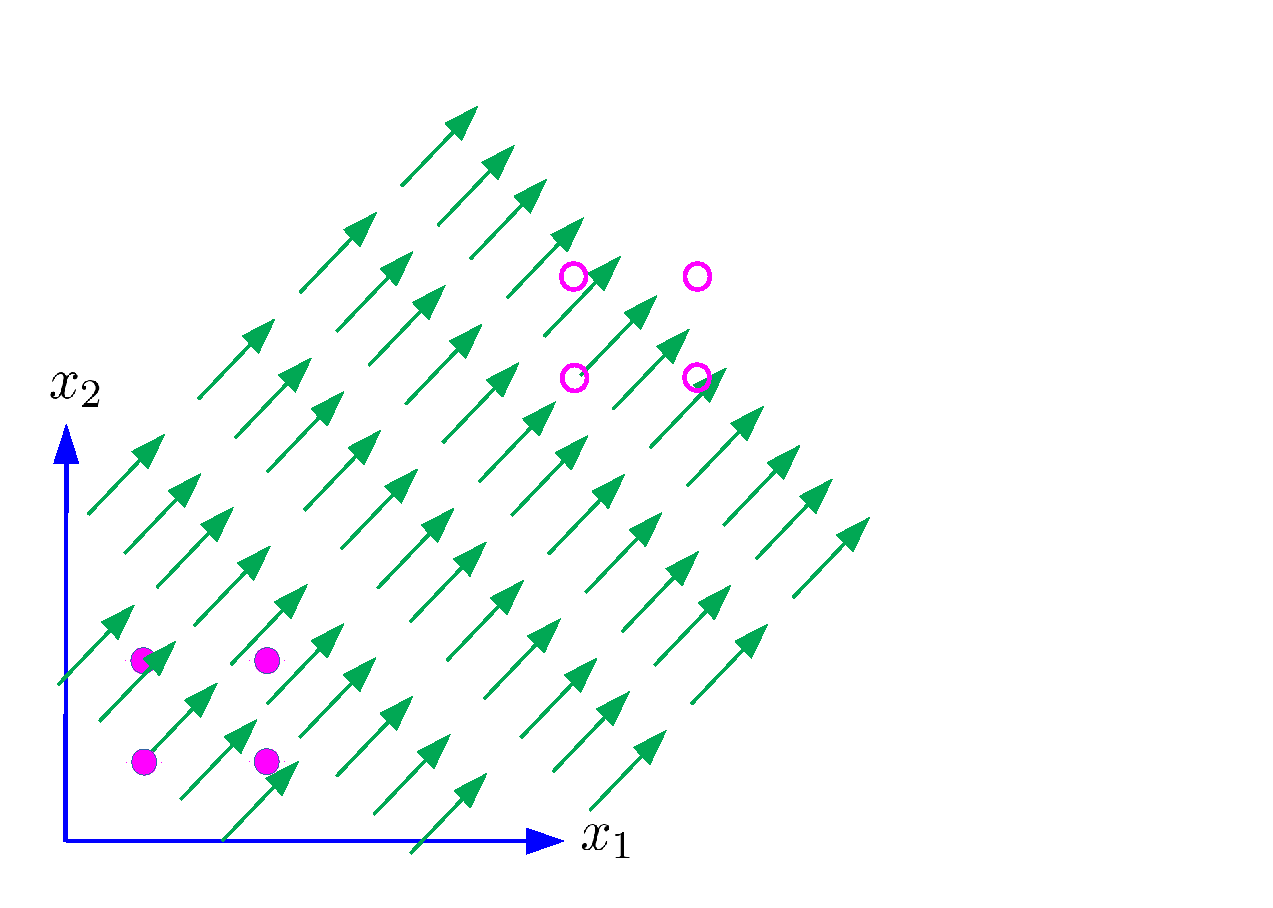
\includegraphics[scale=0.5]{images/c07-CVTranslate3.eps}
 }
\end{center}
\caption{Motion of a control volume due to unidirectional flow}
\label{CVTranslation3}
\end{figure}

% -----------------------------------------------------------------------

\begin{figure}[h]
\begin{center}
\framebox{
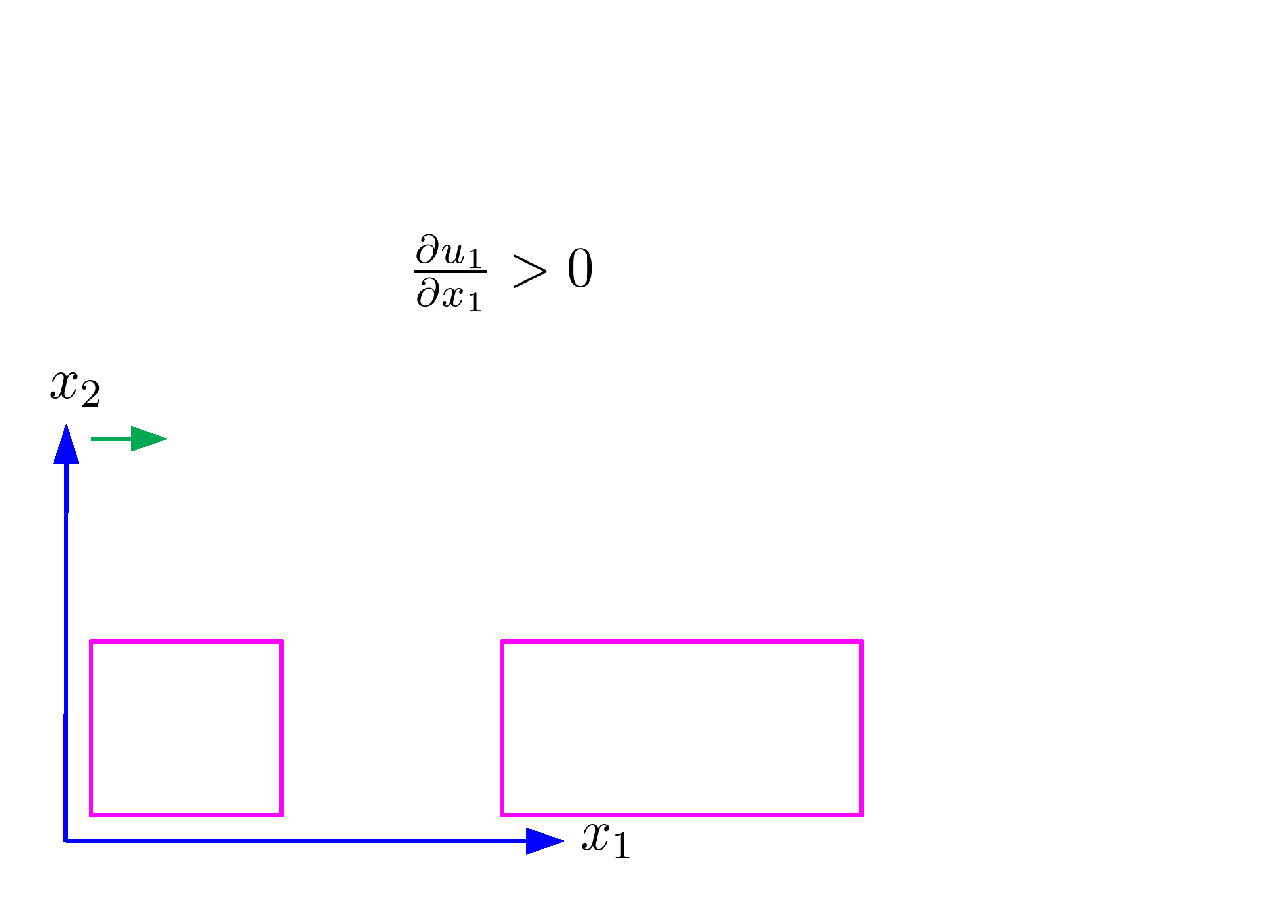
\includegraphics[scale=0.5]{images/c07-CVTranslate4.eps}
 }
\end{center}
\caption{Motion of a control volume due to flow with velocity gradient}
\label{CVTranslation4}
\end{figure}

From the figures, it is clear that uniform velocities lead to only translation of a control volume but velocity gradients would change the shape.

% -----------------------------------------------------------------------

\begin{equation*}
{\partial u_i \over \partial x_j} = 
\left[
\begin{array}{lll}
{\partial u_1 \over \partial x_1} & {\partial u_1 \over \partial x_2} & {\partial u_1 \over \partial x_3} \\
\\
{\partial u_2 \over \partial x_1} & {\partial u_2 \over \partial x_2} & {\partial u_2 \over \partial x_3} \\
\\
{\partial u_3 \over \partial x_1} & {\partial u_3 \over \partial x_2} & {\partial u_3 \over \partial x_3} \\
\end{array}
\right]
\end{equation*}

Changes to a fluid element:
\begin{enumerate}
\item Translation
\item Dilation
\item Shear
\item Rotation
\end{enumerate}

% -----------------------------------------------------------------------

\section{Rate of dilation}

\begin{figure}[h]
\begin{center}
\framebox{
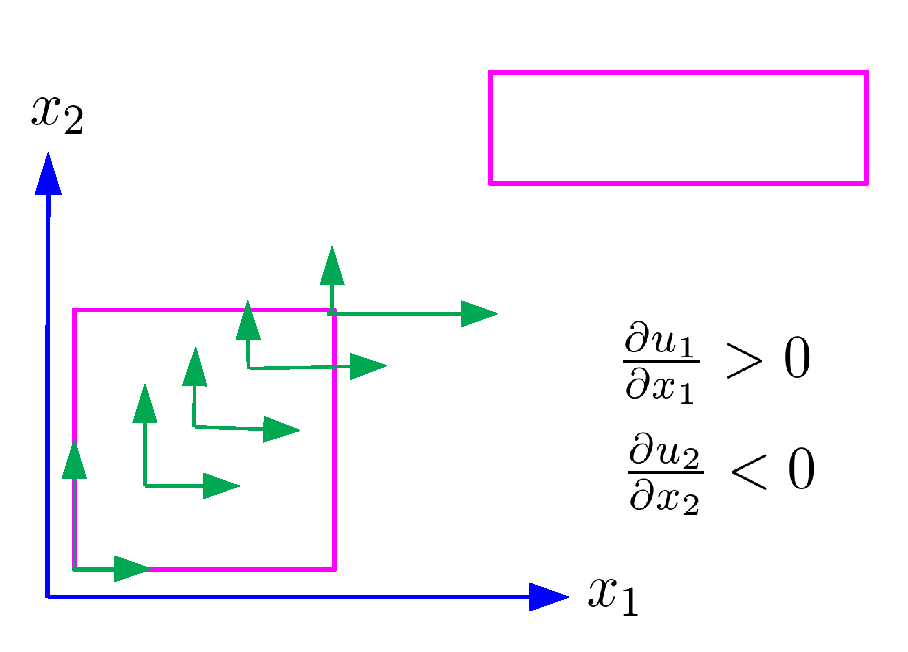
\includegraphics[scale=0.5]{images/c07-CVTranslate5.eps}
 }
\end{center}
\caption{Rate of dilation}
\label{CVTranslation5}
\end{figure}

Define rate of dilation as:
$$ \Delta = \vec{\nabla} \cdot \vec{u} $$
$$ \Delta = \text{Trace of} \, {\partial u_i \over \partial x_j} $$

% -----------------------------------------------------------------------

\section{Other forms of continuity equation}

$$ {1 \over \rho} {D \rho \over D t} + \Delta = 0 $$

We define an {\bf incompressible fluid} as follows:
$$ {1 \over \rho} {D \rho \over D t} = 0 $$

Continuity equation of an incompressible fluid:
$$ \Delta = \vec{\nabla} \cdot \vec{u} = {\partial u_1 \over \partial x_1} + {\partial u_2 \over \partial x_2} + {\partial u_3 \over \partial x_3} = 0 $$

% -----------------------------------------------------------------------

{\bf Continuity equation}: 
For incompressible fluids:
$$\vec{\nabla} \cdot \vec{u} = 0$$

{\bf Statement in words}
Divergence of velocity field is zero

Other coordinate systems such as ($r$, $\theta$, $z$) or ($r$, $\theta$, $\phi$):
\begin{enumerate}
\item Write down velocity field 
\item Look up divergence operator 
\item Express continuity equation
\end{enumerate}

% -----------------------------------------------------------------------


{\bf Continuity equation : cylindrical coordinate system}:

Velocity components:
$$ \vec{V} = V_r \, \hat{e}_r + V_\theta \, \hat{e}_\theta + V_z \, \hat{e}_z $$

$\vec{\nabla}$ operator:
$$ \vec{\nabla} = {\partial \over \partial r} \hat{e}_r + {1 \over r} {\partial \over \partial \theta} \hat{e}_\theta + {\partial \over \partial z} \hat{e}_z $$

Remember:
$$ {\partial \hat{e}_r \over \partial \theta} = \hat{e}_\theta \, \, \& \, \, {\partial \hat{e}_\theta \over \partial \theta} = -\hat{e}_r$$

Continuity equation:
$$ \vec{\nabla} \cdot \vec{V} = {1 \over r} {\partial \over \partial r} \left( r V_r \right) + {1 \over r} {\partial V_\theta \over \partial \theta} + {\partial V_z \over \partial z} = 0 $$


% -----------------------------------------------------

{\bf Continuity equation : spherical coordinate system}:

Velocity components:
$$ \vec{V} = V_r \, \hat{e}_r + V_\theta \, \hat{e}_\theta + V_\phi \, \hat{e}_\phi $$

$\vec{\nabla}$ operator:
$$ \vec{\nabla} = {\partial \over \partial r} \hat{e}_r + {1 \over r} {\partial \over \partial \theta} \hat{e}_\theta + {1 \over r\sin\theta}{\partial \over \partial \phi} \hat{e}_\phi $$

Continuity equation:
$$ \vec{\nabla} \cdot \vec{V} = {1 \over r^2} {\partial \over \partial r} \left( r^2 V_r \right) + {1 \over r \sin\theta} {\partial \over \partial \theta} \left( V_\theta \sin\theta \right) + {1 \over r \sin\theta} {\partial V_\phi \over \partial \phi} = 0 $$


% -----------------------------------------------------

\section{Applications of continuity equation}
Continuity equation for an incompressible fluid:
$$ \vec{\nabla} \cdot \vec{u} = 0 $$
\begin{enumerate}
\item Determine valid unidirectional velocity fields
\item Validate components of a velocity field
\item Determine a velocity components if rest are known
\item For 2D flows, reduce the velocity field to a scalar function
\end{enumerate}

% -----------------------------------------------------

% learning objective
\begin {lo3} [Fluid Flow]
Determine functional form of unidirectional velocity fields
\end {lo3}

\subsection{Unidirectional velocities}

Using the continuity equation for an incompressible fluid, set all velocity components except one as zero and integrate to determine the general form of unidirectional velocity in that direction.

Set $u_2=0$ and $u_3=0$ in the following equation:
$$ {\partial u_1 \over \partial x_1} + {\partial u_2 \over \partial x_2} + {\partial u_3 \over \partial x_3} = 0 $$

The unidirectional velocity along $x_1$ is of the form:
	$$ u_1 = f\left(x_2, x_3 \right) $$

Set two of the three velocity components in the following equation as zero:
$$ {1 \over r} {\partial \over \partial r} \left( r u_r \right) + {1 \over r} {\partial u_\theta \over \partial \theta} + {\partial u_z \over \partial z} = 0 $$

Thus, the unidirectional velocities in cylindrical coordinate system will be of the following forms, along respective directions:
	$$ u_r = {f\left(\theta,z\right) \over r} $$
	$$ u_\theta = f\left(r, z \right) $$
	$$ u_z = f\left(r, \theta \right) $$

% -----------------------------------------------------

Similarly, set two of the three velocity components in the following equation as zero:

$$ {1 \over r^2} {\partial \over \partial r} \left( r^2 u_r \right) + {1 \over r \sin\theta} {\partial \over \partial \theta} \left( u_\theta \sin\theta \right) + {1 \over r \sin\theta} {\partial u_\phi \over \partial \phi} = 0 $$

Thus, the unidirectional velocities in spherical coordinate system will be of the following forms, along respective directions:
	$$ u_r = {f\left(\theta,\phi\right) \over r^2} $$
	$$ u_\phi = f\left(r, \theta \right) $$

% -----------------------------------------------------------------------

% learning objective
\begin {lo3} [Fluid Flow]
Apply continuity equation to validate a velocity field given by its components
\end {lo3}

\subsection{Interpretation of continuity equation}:
Continuity equation for an incompressible fluid in 2D:
$$ {\partial u_1 \over \partial x_1} + {\partial u_2 \over \partial x_2} = 0 $$
\begin{enumerate}
\item If ${\partial u_1 \over \partial x_1} > 0$ then ${\partial u_2 \over \partial x_2} < 0$
\item Increase in magnitude in all directions not possible
\item Flow near corners
\end{enumerate}


% -----------------------------------------------------------------------------------


\section{Summary}

Continuity equation for incompressible flow in rectangular coordinate system is given as: 

$$ {\partial u_x \over \partial x} + {\partial u_y \over \partial y} + {\partial u_z \over \partial z} = 0 $$

Continuity equation for incompressible flow in cylindrical coordinate system is given as: 

$$ {1 \over r} {\partial \left( r V_r \right) \over \partial r} +  {1 \over r} {\partial V_\theta \over \partial \theta} + {\partial V_z \over \partial z} = 0 $$

% -----------------------------------------------------------------------

\section{Exercises}

\begin{question}
\item Which of the following sets of equations represent possible two-dimensional incompressible flow cases?
\begin{enumerate}
	\item $u=2x^2+y^2$; $v=x^3-x(y^2-2y)$
	\item $u=2xy-x^2+y$; $v=2xy-y^2+x^2$
\end{enumerate}
\end{question}
\begin{solution}[print]
Evaluate $\nabla \cdot \vec{u} = 0$ and conclude. 
\end{solution}

% -----------------------------------------------------------------------

\begin{question}
\item Which of the following sets of equations represent possible two-dimensional incompressible flow cases?

\begin{enumerate}
\item $u_r=U\cos\theta$; $u_\theta=-U\sin\theta$
\item $u_r={-q / 2\pi r}$; $u_\theta={K/2\pi r}$
\end{enumerate}
\end{question}
\begin{solution}[print]
\end{solution}

% -----------------------------------------------------------------------

\begin{question}
The $y$ component of velocity in a steady, incompressible flow field in $xy$ plane is $v = {Ay/x^2}$ where $A=2m^2/s$ and $x$ is measured in meters. Find the simplest $y$ component of velocity for this flow field.
\end{question}
\begin{solution}[print]
\end{solution}

% -----------------------------------------------------------------------

\begin{question}
For an incompressible flow in the $r\theta$ plane, the $r$ component of velocity is given as $u_r = -{\lambda \cos\theta/r^2}$. Determine a possible $\theta$ component of velocity. How many possible $\theta$ components are there?
\end{question}
\begin{solution}[print]
\end{solution}
  
% -----------------------------------------------------------------------

\section{Further study}

\begin{enumerate}

\item What is d'Alembert's paradox?
 
\item Watched any NCFMF videos on youtube? Watch one and write down what you have learned. 

\item Have you watched the movie "twister"? Can you try and write down an equation that shows the velocity field of air in a twister?

\end{enumerate}

% -----------------------------------------------------------------------
